%! TEX program = pdflatex
%% Mauricio Caceres Bravo <mauricio.caceres.bravo@gmail.com>

%----------------------------------------------------------------------
\documentclass{article}

\usepackage[summary]{brownpreamble}
\usepackage{etoc}
\setcounter{tocdepth}{2}

\renewcommand{\subsectionmark}[1]{\markboth{#1}{}}
\renewcommand\sectiontype{Lecture \thesection:\ }
\lhead{\color{light-gray} \itshape Math Camp Aug 14, 2023 -- Lecture \thesection}
\rhead{\color{light-gray} \itshape \thesubsection. \leftmark}
% \setcounter{section}{0}
% \renewcommand\SetHideLevel{1pt}
\titleformat{\section}[display]{\sectionstyle}{\sectiontype #1}{0pt}{\vspace{12pt}}

%----------------------------------------------------------------------
\begin{document}
\displayoptions

% ---------------------------------------------------------------------
\section{Proofs, Metric Spaces, Topology}
\label{sec:proofs_metric_spaces_topology}

\localtableofcontents

% ---------------------------------------------------------------------
\subsection{Proofs and Logic}
\label{sub:proofs_and_logic}

Math is a language: It should be possible to express anything you want in math, as you would in English or any other language. However, there are many things that are easier to express in math (just like many things are easier to express in English). One thing that is easier to do in math are proofs.

\subsubsection{If $P$ then $Q$}
\label{ssub:if_p_then_q}

What does it mean?
\begin{itemize}[label=$\bullet$]
  \item Logically, we say $P \implies Q$, that is, ``$P$ implies $Q$'' or ``$P$ therefore $Q$.''
    \begin{figure}[H]
      \centering
      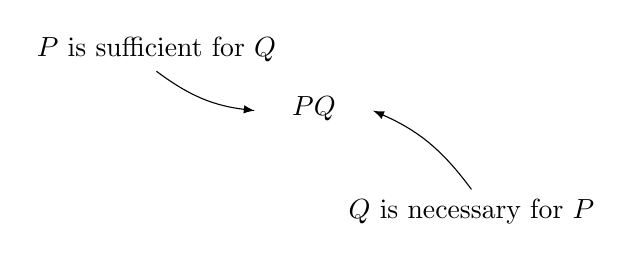
\begin{tikzpicture}[scale=1]
        \draw [->, >=latex]
          (-2, 0.75) to[bend right=15] (-0.75, 0.25)
          node[above] at (-2, 0.75) {$P$ is sufficient for $Q$};
        \draw [->, >=latex]
          (2, -0.75) to[bend right=15] (0.75, 0.25)
          node[below] at (2, -0.75) {$Q$ is necessary for $P$};
        \node[above] at (0, 0) {$P \implies Q$};
      \end{tikzpicture}
    \end{figure}

  \item Graphically we say $P \subseteq Q$
    \begin{figure}[H]
      \centering
      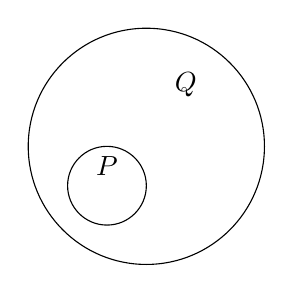
\begin{tikzpicture}[scale=1]
        \draw (0, 0) circle [radius=1.5];
        \draw (-0.5, -0.5) circle [radius=0.5];
        \node[above] at (-0.5, -0.5) {$P$};
        \node[above] at (0.5, 0.5) {$Q$};
      \end{tikzpicture}
    \end{figure}
\end{itemize}

Naturally $P \implies Q \ne Q \implies P$; however, we have that the \keyword{contrapositive} is equivalent, that is,
\[
  P \implies Q \equiv \neg Q \implies \neg P
\]

That is to say, if not $Q$, then not $P$. Logically, if $P \implies Q$ and we do not have $Q$, then we cannot have $P$ (otherwise we'd have $Q$). Graphically, if we are not in $Q$ and $P \subseteq Q$, then we cannot be in $P$.

\subsubsection{Proof Strategies}
\label{ssub:proof_strategies}

\begin{enumerate}
  \item \keyword{Direct}: Show $P \implies Q$. That is, find some path of logical statements that leads from $P$ to $Q$.
    \begin{example}
      Show $m \in \mathbb{Z}$ even $\implies p \cdot m$ even $\forall p \in \mathbb{Z}$. $m$ is even $\iff \exists q \in \mathbb{Z}$ s.t. $m = 2q$, hence $pm = 2pq$. Last, $pq \in \mathbb{Z}$, so $pm$ equals an integer times $2$, implying $pm$ is even.
    \end{example}

  \item \keyword{Contrapositive}: Show $\neg Q \implies \neg P$. This is very similar to a direct proof, but often it is useful to rephrase what we want to show in its contrapositive form. Further, texts will, at times, proceed by contrapositive without making explicit mention that is what they are doing.

  \item \keyword{Contradiction}: If $\neg P$ leads to $Q$ and $Q$ is false, then $P$ must be true.
    \begin{example}
      One of the most famous proofs by contradiction is that $\sqrt{2} \notin \mathbb{Q}$. Suppose the negation of that statement is true, that is, $\sqrt{2} \in \mathbb{Q}$. Recall
      \[
        \mathbb{Q} = \Fset{
          p / q: (p, q) \in \mathbb{Z} \times \mathbb{Z}\setminus\set{0}
        }
      \]

      Hence $\exists p, q$ co-prime s.t. $\sqrt{2} = p / q$. (\NB: If $p, q$ are not co-prime then the fraction can be simplified until we find $p, q$ co-prime.\footnote{Let $\sqrt{2} = \widetilde{p} / \widetilde{q}$ for any $\widetilde{p}, \widetilde{q}$ and let $m$ be the product of all their co-factors; $p \equiv \widetilde{p} / m, q \equiv \widetilde{q} / m$ gives $\sqrt{2} = p / q$ with $p, q$ co-prime.}) Note
      \[
        \sqrt{2} = \dfrac{p}{q}
        \iff
        -2 = \dfrac{p^2}{q^2}
        \quad
        \text{or}
        \quad
        2 = \dfrac{p^2}{q^2}
      \]

      WLOG\footnote{WLOG means ``Without Loss of Generality.'' This is occasionally used in proofs in order to shorten them: This means that even through there is more than one case to consider, proving any of them would follow identical steps to the one you are about to show; hence despite focusing on a specific case, the proof has not lost its general applicability (its generality).} take the positive root, so
      \[
        2 = \dfrac{p^2}{q^2}
        \implies
        2q^2 = p^2
        \implies
        p^2 \text{ is even }
        \implies
        p \text{ is even }
        \implies
        \exists m \in \mathbb{Z}: p = 2m
      \]

      Thus
      \[
        2q^2 = (2m)^2
        \iff
        q^2 = 2m^2
        \implies
        q^2 \text{ is even }
        \implies
        q \text{ is even }
        \implies
        \exists n \in \mathbb{Z}: q = 2n
      \]

      Hence $p, q$ are both divisible by $2$ and are not co-primes, contradiction.
    \end{example}

    There is a very slight nuance with the proof above involving special cases. Can you spot it?\footnote{I believe the common definition of co-prime integers does not preclude both integers from being equal to $1$, in which case my subsequent claims about $p, q$ being even do not hold. We can readily see that $p = 1$ is an issue since $2 = 1/q^2 \le 1$ is already a contradiction; however, a more subtle case is when $q = 1$, which which case $2 = p^2$, contradiction since $p \in \mathbb{Z}$.}

  \item \keyword{Induction}: We want to say something about statements that can be indexed by the natural numbers. Using induction we do that in two steps:
    \begin{enumerate}[a)]
      \item Prove the \keyword{base step}, $P(1)$, is true.

      \item Prove the \keyword{inductive step}, $P(k) \implies P(k + 1)$, is true (i.e. assume $P(k)$ is true and show $P(k + 1)$).
        \begin{example}
          We want to show the sum of the first $k$ odd numbers is $k^2$, that is:
          \[
            \sum^{k}_{i = 1} 2i - 1 = k^2
          \]

          For the base step we can see $1 = 1^2$. For the inductive step, assume $P(k)$ is true and show $P(k + 1)$:
          \[
            \sum^{k + 1}_{i = 1} 2i - 1
            =
            \sum^{k}_{i = 1} 2i - 1
            +
            2(k + 1) - 1
            \stackrel{!}{=}
            k^2
            +
            2k
            +
            1
            =
            (k +  1)^2
          \]

          where $\stackrel{!}{=}$ is true by the inductive step assumption (i.e. $P(k)$ means $\sum^{k}_{i = 1} 2i - 1 = k^2$).
        \end{example}

        In case you are curious, here's a proof with a tricky base step. Straight from \href{https://en.wikipedia.org/wiki/Mathematical_induction#Base_case_other_than_0_or_1}{Wikipedia \ExternalLink}:
        \begin{example}
          Prove that $\forall k \ge 12 ~~ \exists m, n \in \mathbb{Z}_+$ (non-negative integers) s.t. $4m + 5n = k$.
          \begin{enumerate}[a)]
            \item Base: $k = 12$ then $m = 3, n = 0$.
            \item Induction: Assume $\exists m_k, n_k$ s.t. $4m_k + 5n_k = k$ and show $\exists m_{k + 1}, n_{k + 1}$ s.t. $4m_{k + 1} + 5n_{k + 1} = k + 1$.
              \begin{align*}
                k + 1
                = 4m_k + 5n_k + 1
                = 4m_k + 5n_k + 5 - 4
                = 4(m_k - 1) + 5(n_k + 1)
              \end{align*}

              Hence $m_{k + 1} = m_k - 1, n_{k + 1} = n_k + 1$ if $m_k > 0$. If $m_k = 0$, then $n_k \ge 3$, so
              \begin{align*}
                k + 1
                = 4m_k + 5n_k + 1
                = 4m_k + 5n_k + 16 - 15
                = 4(m_k + 4) + 5(n_k - 3)
              \end{align*}

              and $m_{k + 1} = m_k + 4, n_{k + 1} = n_k - 3$.
          \end{enumerate}

          Note for several $k < 12$ this cannot be true (e.g. $k = 3$).
        \end{example}
    \end{enumerate}
\end{enumerate}

% ---------------------------------------------------------------------
\subsection{Functions}
\label{sub:functions}

We will not delve into set theory. Intuitively, we can think of a set as a collection of (unique) elements, and we can think of functions as rules that associate every element in one set with an element in another set.\footnote{Formally, we can define a function $f$ from $X$ to $Y$ as a binary relation s.t. $f \subseteq (X \times Y)$ and for each element $x \in X$ there is one (and only one) element $y \in Y$ s.t. $(x, y) \in f$ (though for each element in $y$ there may be some $z \ne x$ s.t. $(z, y) \in f$). Chapter 1 of Ok has a rigorous treatment of functions following an introduction to set theory.}
\begin{definition}[function]\label{def:lecture1_functions}
  $f$ is a \keyword{function} with \keyword{domain} $X$ mapping to a \keyword{co-domain} $Y$ if for every element $x \in X$ there exists a $y \in Y$ s.t. $f(x) = y$. We write $f: X \to Y$, and for any $S \subseteq X$
\[
  f(S) = \Fset{y \in Y: \exists x \in S ~~\text{s.t.}~~ f(x) = y}
\]

  is the \keyword{image} of $S$ under $f$. $f(X)$, the image of the domain, is called the \keyword{range}: The set of points in $Y$ at least some element of $X$ is mapped into.
\end{definition}

\begin{definition}[inverse image]\label{def:lecture1_inverse_image}
  If $f: X \to Y$ then for any $S \subseteq Y$ the \keyword{inverse image} of $S$ is
  \[
    f^{-1}(S) = \Fset{
      x \in X: \exists y \in Y ~~\text{s.t.}~~ f(x) = y
    }
  \]
\end{definition}

\begin{remark}
  The inverse image is distinct from the concept of an inverse function. A function is invertible if $\exists g$ s.t. $f(x) = y \iff g(y) = x$; this is also denoted $g = f^{-1}$ because the image of the inverse is the inverse image. However, functions needn't be invertible, while the inverse image is always defined.
\end{remark}

In general it need not be the case that $f(X) = Y$, since some points of $Y$ might not be mapped into. Further, a single point in $Y$ might be the mapping of several points in $X$. We have some special interest in functions for which that is not the case.
\begin{definition}[injective]\label{def:lecture1_injective}
  A function $f: X \to Y$ is \keyword{injective} (or one-to-one) if $f(x) = f(y) \implies x = y$.
\end{definition}

\begin{definition}[surjective]\label{def:lecture1_surjective}
  $f$ is \keyword{surjective} (or onto) if $f(X) = Y$.
\end{definition}

\begin{definition}[bijective]\label{def:lecture1_bijective}
  $f$ is \keyword{bijective} or a bijection if it is injective and surjective.
\end{definition}

% ---------------------------------------------------------------------
\subsection{Countability}
\label{sub:countability}

\begin{definition}[countability]\label{def:lecture1_countable}
  A set $X$ is \keyword{countably infinite} or \keyword{countable} if $\exists$ a bijection from $X$ to the natural numbers $\mathbb{N}$.
\end{definition}

We make a distinction between finite and countable (note finite sets are not countable by the above definitions). Some examples of countably infinite sets:
\begin{enumerate}
  \item $\mathbb{N}$ is countable since a bijection from $\mathbb{N} \to \mathbb{N}$ is given by the identity $f(x) = x$.

  \item $\mathbb{Z}$ is countable. This is slightly more complicated but we can enumerate all the integers:
    \[
      \Fset{0, -1, 1, -2, 2, \ldots}
    \]

    This is the enumeration given by the bijection $f(x) = 2|x| - 1(x < 0)$.
\end{enumerate}

Is $\mathbb{Q}$ countable? Is $\mathbb{R}$? The answers are yes and no, respectively, but the arguments are more nuanced.
\begin{claim}
  $\mathbb{Q}$ is countable.
\end{claim}

\begin{proof}
  Note $X$ is countable if $\exists$ an injection $f: X \to \mathbb{N}$. Suppose there exists such an injection, so $f(X) \subseteq \mathbb{N}$. Denote the elements of this set $\set{n_1, n_2, n_3, \ldots}$ and note $\exists$ unique $x \in X$ for each element s.t. $f(x_{n_i}) = n_i$ for each $i \in \mathbb{N}$. Define $g(x_{n_i}) = i$ and we have $g: X \to \mathbb{N}$ is a bijection, so $X$ is countable by definition.

  An immediate corollary is that if $X$ is countable and $S \subseteq X$ then $S$ is countable (or finite), as the bijection defined over $X$ would still be an injection when restricted to $S$. Now to show $\mathbb{Q}$ is countable, consider $g(p, q) = p / q$ defined over the set $\mathbb{Z} \times \mathbb{Z}\setminus\set{0}$. We can see $\mathbb{Q} = g(\mathbb{Z} \times \mathbb{Z}\setminus\set{0})$, and $g^{-1}(\mathbb{Q}) \subseteq \mathbb{Z} \times \mathbb{Z}$. If we can show $\mathbb{Z} \times \mathbb{Z}$ is countable, it should follow $\mathbb{Q}$ is countable.

  Take any sets $P, Q$ countable; we can enumerate their elements as
  \[
    P = \Fset{p_1, p_2, \ldots}
    \quad
    \text{and}
    \quad
    Q = \Fset{q_1, q_2, \ldots}
  \]

  and we can enumerate their Cartesian product as
  \[
    \begin{matrix}
      Q \times P & p_1 & p_2 & p_3    & p_4    & \ldots \\
      q_1        & 1   & 3   & 6      & 10     &        \\
      q_2        & 2   & 5   & 9      &        &        \\
      q_3        & 4   & 8   & \ddots &        &        \\
      q_4        & 7   &     &        & \ddots &        \\
      \vdots
    \end{matrix}
  \]

  meaning $P \times Q$ is countable. The bijection that corresponds to that table is
  \begin{align*}
    f(p_i, q_j) = \dfrac{(i + j - 1)(i + j)}{2} - (i - 1)
  \end{align*}
\end{proof}

\begin{claim}
  $\mathbb{R}$ is \textbf{\textit{not}} countable.
\end{claim}

\begin{proof}[Cantor's Diagonal Argument]
  We proceed by contradiction.\footnote{Cantor's diagonalization proof has been called one of the most beautiful proofs in mathematics.} Suppose $\mathbb{R}$ is countable, so we can enumerate its elements as $\mathbb{R} = \set{r_1, r_2, \ldots}$. The decimal representation of each element in $\mathbb{R}$ is then
  \begin{align*}
    r_1 & = N_1.x_{11}x_{12}x_{13}\ldots \\
    r_2 & = N_2.x_{21}x_{22}x_{23}\ldots \\
    r_3 & = N_3.x_{31}x_{32}x_{33}\ldots \\
    \vdots
  \end{align*}

  where $N_i \in \mathbb{Z}$ and $x_{ij} \in \set{0, \ldots, 9}$. Take $y = N.y_1y_2y_3\ldots$ s.t. $y_i \ne x_{ii}$ and $y$ doesn't have an alternative representation (so $y$ doesn't end in all $0$s or all $9$s; but we can do this, since for any $x_{ii}$ we have $7$ numbers to choose from other than $0, 9$, or $x_{ii}$). $y \in \mathbb{R}$ but $y \ne r_j$ for any $j$, contradiction. (Cantor actually did this proof for just the real interval $[0, 1]$; can you see why that's sufficient?)
\end{proof}

Why doesn't this proof work for $\mathbb{Q}$?\footnote{If we try to use that same proof to show $\mathbb{Q}$ is not countable there is actually no guarantee that the number $y$ we construct will be an element of $\mathbb{Q}$. We have already established there are numbers that are not in $\mathbb{Q}$, whereas $\mathbb{R}$ is actually defined to be complete (this is a formal term, but intuitively it means that $\mathbb{R}$ has \textit{all} the numbers).}

\begin{tacomment}{1}
  While we often work with $\mathbb{R}$, the real numbers aren't actually in reality. We made them up. There is no such thing as $\pi$ pies: Even at the sub-atomic level, there will be a finite number of atoms, and any numbers we derive will be integers or rationals.

  Furthermore, it is not obvious what it means to make choices from uncountable sets.  Of course we can make a choice from a set that is uncountable, you might think: It has infinitely many more elements than a countable set! It seems trivial, but if we are not careful we end up with some rather unintuitive paradoxes.

  For example, a consequence of the axiom of choice (which allows us to make a choice out of uncountable sets in an intuitive way) is the Banach-Tarski paradox: Take any ball in 3-dimensional space (or higher); we can partition the ball into finitely many pieces and rearrange (move and rotate) those pieces into two balls identical to the first one.

  So in general it will be useful to think of statements that are true for $\mathbb{R}$ as being the convenient version of something that we should be able to show in $\mathbb{Q}$. We will see later on that while $\mathbb{R}$ is infinitely larger than $\mathbb{Q}$, the rational numbers are \keyword{dense} in the reals. Informally, $\forall a, b \in \mathbb{R} ~~ \exists q \in Q$ s.t.
  \[
    a < q < b
  \]

  whenever $a < b$. (``Informally'' because the concept of density here depends on the order, $<$, and in general we will be able to define that being dense means without it.)
\end{tacomment}

\begin{remark}
  The finite Cartesian product of countable sets was countable, which we can show by induction. The claim is that if $P$ is countable, then $P^N$ is also countable. This is another example of induction where the base step cannot be $N = 1$ (since this ``base'' step is actually given by the premise of the problem).
  \begin{enumerate}[a)]
    \item Base: $P \times P$ is countable. We proved the Cartesian product of \textit{two} countable sets is countables.

    \item Induction: If $P^N$ is countable then $P^{N + 1} = P^N \times P$ is the product of two countable sets, which, again, we already showed is countable (the induction assumption gets $P^N$ is countable and the problem statement gives that $P$ itself is countable).
  \end{enumerate}

  In this case, the base was $N = 2$.
\end{remark}

% ---------------------------------------------------------------------
\subsection{Metric Spaces}
\label{sub:metric_spaces}

\begin{definition}[distance]\label{def:lecture1_distance}
  A function $d: X \times X \to \mathbb{R}_+$ with $X \ne \varnothing$ is called a \keyword{distance} or \keyword{metric} on $X$ if $\forall x, y, z \in X$
  \begin{enumerate}
    \item $d(x, y) = 0 \iff x = y$,

    \item $d(x, y) = d(y, x)$ (it is symmetric), and

    \item $d(x, y) \le d(x, z) + d(z, y)$ (the triangle inequality holds).
  \end{enumerate}
\end{definition}

Note the triangle inequality says that tou cannot ``shorten'' the distance between two points if you first ``stop by'' a third point. It might be equal (if $z$ happens to be in the ``path'' from $x$ to $y$, for some definition of ``path'') but it can never be strictly smaller. Last, note we defined $d$ to be $\ge 0$ for all $x, y$ in the space.

\begin{definition}[metric space]\label{def:lecture1_space}
  A \keyword{metric space} $(X, d)$ is a non-empty set $X$ with a metric $d$ defined on $X$.
\end{definition}

Some examples of metric spaces:
\begin{enumerate}
  \item For any $X \ne \varnothing$, one way to metricize the space is the discrete metric
    \begin{align*}
      d(x, y) = \begin{cases}
        1 & x \ne y \\
        0 & x = y
      \end{cases}
    \end{align*}

  \item $\mathbb{R}^N$ with the euclidean distance,
    \begin{align*}
      d(x, y)
      = \norm{x - y}
      = \sqrt{\sum^{N}_{i = 1} (x_i - y_i)^2}
    \end{align*}

  \item More generally, consider for $1 \le p \le \infty$ the distance on $\mathbb{R}^N$ for $N \in \mathbb{N}$
    \begin{align*}
      d_p(x, y)
      =
      \begin{cases}
        \left(\displaystyle\sum^{N}_{i = 1} |x_i - y_i|^p\right)^{1 / p}
          & 1 \le p < \infty \\[12pt]
        \displaystyle\max_{i = 1, \ldots, N} |x_i - y_i|
          & p = \infty
      \end{cases}
    \end{align*}

    $(\mathbb{R}^N, d_p)$ is a metric space, often called a $L^p$-space.\footnote{\NB: I have encountered the terminology $L^p$ to refer to both the metric $d_p$ as well as the space $(\mathbb{R}^N, d_p)$.} $d_2$ is the euclidean distance, but it turns out that, while geometrically intuitive, it's not necessary to preserve a lot of the properties we care about.
    \begin{figure}[H]
      \centering
      \caption{Unit ``circle'' in $\mathbb{R}^2$ under different $d_p$ metrics}
      \label{fig:unit_circle_in_r_2_under_different_d_p_metrics}
      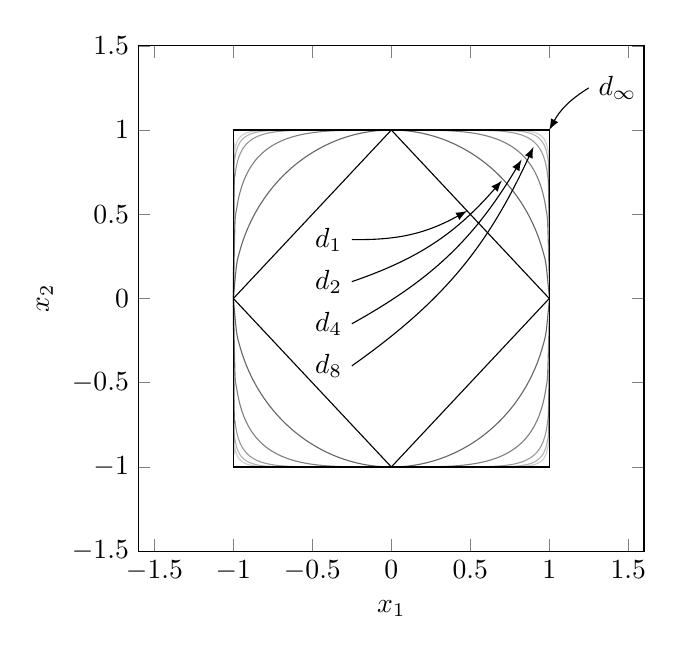
\begin{tikzpicture}
        \begin{axis}[name=plot1
          %,title=
          ,width=8cm
          ,height=8cm
          ,ymin=-1.5
          ,ymax=1.5
          ,xmin=-1.6
          ,xmax=1.6
          ,domain=-1:1
          ,ylabel=$x_2$
          ,xlabel=$x_1$
        ]
        % around 0
        % y = (1 - x^p)^(1/p)
        \addplot [smooth, samples = 100, domain=0:1] {abs(1 - x)};
        \addplot [smooth, samples = 100, domain=-1:0] {abs(x + 1)};
        \addplot [smooth, samples = 100, opacity=0.6] {(1 - x^2)^(1/2)};
        \addplot [smooth, samples = 200, opacity=0.5] {(1 - x^4)^(1/4)};
        \addplot [smooth, samples = 400, opacity=0.4] {(1 - x^8)^(1/8)};
        \addplot [smooth, samples = 400, opacity=0.3] {(1 - x^12)^(1/12)};
        \addplot [smooth, samples = 400, opacity=0.2] {(1 - x^16)^(1/16)};

        \addplot [smooth, samples = 100, domain=0:1] {-abs(1 - x)};
        \addplot [smooth, samples = 100, domain=-1:0] {-abs(x + 1)};
        \addplot [smooth, samples = 100, opacity=0.6] {-(1 - x^2)^(1/2)};
        \addplot [smooth, samples = 200, opacity=0.5] {-(1 - x^4)^(1/4)};
        \addplot [smooth, samples = 400, opacity=0.4] {-(1 - x^8)^(1/8)};
        \addplot [smooth, samples = 400, opacity=0.3] {-(1 - x^12)^(1/12)};
        \addplot [smooth, samples = 400, opacity=0.2] {-(1 - x^16)^(1/16)};

        \draw [->, >=latex] (axis cs:-0.25,  0.35) to[bend right=15] (axis cs:0.48,  0.52);
        \draw [->, >=latex] (axis cs:-0.25,  0.10) to[bend right=15] (axis cs:0.7,   0.7);
        \draw [->, >=latex] (axis cs:-0.25, -0.15) to[bend right=15] (axis cs:0.825, 0.825);
        \draw [->, >=latex] (axis cs:-0.25, -0.40) to[bend right=15] (axis cs:0.9,   0.9);
        \draw [->, >=latex] (axis cs:1.25, 1.25) to[bend right=15] (axis cs:1, 1);

        \node[left] at (axis cs:-0.25,  0.35) {$d_1$};
        \node[left] at (axis cs:-0.25,  0.10) {$d_2$};
        \node[left] at (axis cs:-0.25, -0.15) {$d_4$};
        \node[left] at (axis cs:-0.25, -0.40) {$d_8$};

        \node[right] at (axis cs:1.25, 1.25) {$d_{\infty}$};
        \draw [-]
          (axis cs:-1, -1) --
          (axis cs:-1,  1) --
          (axis cs: 1,  1) --
          (axis cs: 1, -1) --
          (axis cs:-1, -1)
        ;
        \end{axis}
      \end{tikzpicture}
    \end{figure}

    In the figure above we can get some intuition for why we defined the $d_{\infty}$ metric as the max; graphically on $\mathbb{R}^2$, we can see this is the natural extension of $d_p$ as $p \to \infty$.
\end{enumerate}

While it can be useful to develop an abstract understanding of metric spaces, for the purposes of this class it's fine if you think of metric spaces as Euclidean space (i.e. $(\mathbb{R}^N, d_2)$, which I will simply denote as $\mathbb{R}^N$).
\begin{remark}
  What is the intuition for $d_p$ metrics?
  \begin{itemize}[label=$\bullet$]
    \item $d_2$ is the Euclidean distance, the ``straight line'' between two points.

    \item $d_{\infty}$ is the largest distance.

    \item $d_1$ is the sum of the absolute differences.
  \end{itemize}

  You don't really have to worry too much about $d_p$ in this class, and it's probably unlikely you'll see them outside of math class. It does bridge the gap between $d_1$ and $d_{\infty}$, and it can generate curvatures that might be of interest in some applications.
\end{remark}

% ---------------------------------------------------------------------
\subsection{Introduction to Topology}
\label{sub:introduction_to_topology}

\begin{definition}[$\varepsilon$-neighborhood]\label{def:lecture1_neighborhood}
  Let $X$ be a metric space. For each $x \in X$ we define the \keyword{$\varepsilon$-neighborhood} of $x$ as
  \[
    N_{\varepsilon, X}(x) = \Fset{y \in X: d(x, y) < \varepsilon}
  \]
\end{definition}

On $\mathbb{R}$, we can see this is just the interval of length $2\varepsilon$ centered around $x$; on $\mathbb{R}^2$ this is a circle, on $\mathbb{R}^3$ it is a ball, and so on. Neighborhoods are never empty, since at least $x \in N_{\varepsilon, X}(x)$.
\begin{remark}
  In Euclidean space an $\varepsilon$-neighborhood is called an \keyword{$\varepsilon$-ball}. Henceforth we will use $\varepsilon$-balls in place of neighborhoods, denoting the $\varepsilon$-ball centered around a point $x$ as $B_{\varepsilon}(x)$:
  \[
    B_{\varepsilon}(x) = \Fset{y \in X: \Fnorm{x - y} < \varepsilon}
  \]

  However, know the results we discuss hold more generally for metric spaces and neighborhoods.
\end{remark}

\begin{definition}[open]\label{def:lecture1_open_set}
  Let $S \subseteq \mathbb{R}^{N}$; $S$ is \keyword{open} in $\mathbb{R}^N$ if $\forall s \in S ~~ \exists \varepsilon > 0$ s.t. $B_{\varepsilon}(x) \subseteq S$.
\end{definition}

\begin{definition}[closed]\label{def:lecture1_closed_set}
  Let $S \subseteq \mathbb{R}^{N}$; $S$ is \keyword{closed} if its complement $S^C = \mathbb{R}^N \setminus S$ is open.
\end{definition}

Some examples of open and closed sets:\footnote{Note the definition of openness uses $\subseteq$ instead of $\subset$. This can be an important distinction, and gets to the fact openness and closeness are not intrinsic properties of subsets: They are tied to the set they are defined in as well as the metric that has been defined on the space. Similarly, a set is defined as closed if its complement \textit{in a given space} is open. All this might make you suspect that sets can be both open or closed if we simply change what they are open or closed relative to, and you would be right!}
\begin{enumerate}
  \item The interval $(0, 1)$ in $\mathbb{R}$ is open. Take any $0 < x < 1$ and let
    \begin{align*}
      \varepsilon \equiv \min\Fset{x - 0.5 (0 + x), 0.5 (1 - x))}
    \end{align*}

    Note $B_{\varepsilon}(x) = (x - \varepsilon, x + \varepsilon)$, so $0 < 0.5x \le x - \varepsilon < x < x + \varepsilon \le 0.5(1 + x) < 1$, means $B_{\varepsilon}(x) \subseteq (0, 1)$.

  \item The interval $[0, 1]$ is closed in $\mathbb{R}$. $(-\infty, 0)$ is open. For any $x < 0$, take $\varepsilon = |x| / 2$ and we have $-\infty < x - \varepsilon < x < x + \varepsilon < 0$. Similarly, for $x > 1$ take $\varepsilon = (x + 1) / 2$ and we get $1 < x - \varepsilon < x < x + \varepsilon < \infty$. Since its complement is open, $[0, 1]$ is closed.

  \item The interval $[0, 1)$ is open in $\mathbb{R}_+$. This is a bit less obvious. $[0, 1)$ is not open in $\mathbb{R}$ because if we take $x = 0$, any $\varepsilon > 0$ gives $x - \varepsilon < 0$, and thus the $\varepsilon$-neighborhood is not in $[0, 1)$. However, in $\mathbb{R}_+$ there are no points $< 0$, so there is nothing to contradict $[0, 1)$ being open.

    What about $[0, 1)$ in $\mathbb{R}$? Is it open or closed?\footnote{It's actually neither.}
\end{enumerate}

\begin{claim}
  The empty set $\varnothing$ and the entire space $\mathbb{R}^N$ are both open and closed.
\end{claim}

\begin{proof}
  The complement of  the empty set is $\mathbb{R}^N \setminus \varnothing = \mathbb{R}^N$, the entire space itself. Take any $x \in \mathbb{R}^N$ and any finite $\varepsilon > 0$; by definition $B_{\varepsilon}(x) \subseteq \mathbb{R}^N$, so $\mathbb{R}^N$ is open, and $\varnothing$ is closed.

  The empty set is open by vacuity: Pick $\varepsilon > 0$ and any $x \in \varnothing$; we have $B_{\varepsilon}(x) = \varnothing \subseteq \varnothing$. Albeit correct, I'll admit this is not  the most intuitive argument. By contradiction, if $\varnothing$ is not open $\exists x \in \varnothing, \varepsilon > 0, y \in B_{\varepsilon}(x)$ s.t. $y \notin \varnothing$. However, $\varnothing$ is empty, so $x \in \varnothing$ is a contradiction. Since the empty set is open, $\mathbb{R}^N$ is closed, completing the proof.
\end{proof}

Can you prove that $\varepsilon$-balls are open?\footnote{Hint: You can use the triangle inequality.}
\begin{claim}
  \begin{itemize}[label=$\bullet$]
    \item Any union of open sets is open.

    \item A finite intersection of open sets is open.

    \item Any intersection of closed sets is closed.

    \item A finite union of closed sets is closed.
  \end{itemize}
\end{claim}

To see why we require a finite intersection for open sets, consider $I_n = (-1/n, 1/n)$ in $\mathbb{R}$. Each set is open, but $\bigcap^{\infty}_{n = 1} I_n = \set{0}$, and singletons are closed in $\mathbb{R}$, so the infinite intersection is closed. Similarly, we can see why we need a finite union for closed sets: $\bigcup_{x \in (0, 1)} \set{x} = (0, 1)$; we just discussed how singletons are closed, but the infinite union can be open.
\begin{definition}[interior, closure, boundary]\label{def:lecture1_interior_closure_boundary}
  \begin{enumerate}
    \item The union of every open set $O$ s.t. $O \subseteq S$ is the \keyword{interior} of $S$. We denote it as $\interior(S)$.

    \item The intersection of every closed set $K$ s.t. $S \subseteq K$ is the \keyword{closure} of $S$. We denote it as $\closure(S)$.

    \item The \keyword{boundary} of $S$ is the set difference between the closure and the interior, $\boundary(S) = \closure(S) \setminus \interior(S)$.
  \end{enumerate}
\end{definition}

\begin{claim}
  An open set is its own interior. A closed set is its own closure.
\end{claim}

The interior is always open, since arbitrary unions of open sets are open; similarly, the closure is always closed, since arbitrary intersections of closed sets are closed.
\begin{definition}
  Let $S \subseteq \mathbb{R}^N$; $S$ is \keyword{bounded} if $\exists \varepsilon > 0, s \in S$ s.t. $S \subseteq B_{\varepsilon}(x)$.
\end{definition}

\begin{definition}
  Let $S \subseteq \mathbb{R}$; $a$ is an \keyword{upper bound} for $S$ if $\forall s \in S$ we have $s \le a$. The least upper bound is called the \keyword{supremum}, denoted $\sup S$.
\end{definition}

\begin{definition}
  Let $S \subseteq \mathbb{R}$; $b$ is an \keyword{lower bound} for $S$ if $\forall s \in S$ we have $s \ge b$. The greatest lower bound is called the \keyword{infimum}, denoted $\inf S$.
\end{definition}

\begin{claim}
  Let $S \subseteq \mathbb{R}$. $a = \sup S$ iff $a$ is an upper bound s.t. $~ \forall c < a ~~ \exists s \in S$ s.t. $c < s$; similarly, $b = \inf S$ iff $b$ is a lower bound s.t. $~ \forall c > b ~~ \exists s \in S$ s.t. $c > s$.
\end{claim}

\begin{remark}
  In class I got myself twisted with this proof, and it's because I mis-remembered the premise! The characterization is as stated above, but mid-proof I hallucinated that $c \in S$ was also a requirement, which would make the equivalency false. The proof I gave in class is actually a more complicated version of the one below that still relied on $c$ being arbitrary and not necessarily inside the set. The below is simpler!
\end{remark}

\begin{proof}
  Let $a = \sup S$ and take any $c \in S$ s.t. $c < a$. By contradiction suppose $\forall s \in S$ we have $s \le c < a$, so $c$ is an upper bound smaller than $a$, which contradicts the definition of the $\sup$. Now let $a$ be an upper bound s.t. for any $c \in S$ with $c < a$ there exists some $s \in S$ s.t. $c < s$. By contradiction, if $a \ne \sup S$ then by definition of the $\sup$ it must be that $\sup(S) < a$; however, by premise we now have $\exists s \in S$ s.t. $\sup S < s$, which contradicts the definition of the $\sup$. Hence $a = \sup S$.

  The arguments for the $\inf$ are entirely analogous.
\end{proof}

\begin{remark}
  For any $S \subseteq \mathbb{R}$ that is bounded above, $\sup S \in \mathbb{R}$; similarly, for any $S \subseteq \mathbb{R}$ that is bounded below, $\inf S \in \mathbb{R}$. This is not obvious as, for example, the set $\mathbb{Q} \cap (-\pi, \pi)$ does not have a $\sup$ or an $\inf$ in $\mathbb{Q}$. The fact this is true in $\mathbb{R}$ is a consequence of a property called ``completeness.'' We will not discuss it in depth in this class, but intuitively it means that $\mathbb{R}$ has no ``holes'' (unlike, say, $\mathbb{Q}$). The real line $\mathbb{R}$ is actually constructed to have this property, and you may encounter references to the \textit{completeness axiom}.
\end{remark}

\begin{definitionx}[Archimedean Property]\label{def:lecture1_archimedean}
  $\forall \varepsilon > 0 ~~ \exists N \in \mathbb{N}$ s.t. $0 < 1/N < \varepsilon$.
\end{definitionx}

\begin{claim}
  $\mathbb{Q}$ is \keyword{dense} in $\mathbb{R}$. In this context, $\forall a, b \in \mathbb{R}$ s.t. $a < b ~~ \exists q \in \mathbb{Q}$ s.t. $a < q < b$.
\end{claim}

\begin{proof}
  Density is defined as a more general property of metric spaces, but in the context of the real line the above is a good characterization: You can always find a rational number between any two real numbers.  Since $b - a > 0$, the \nameref{def:lecture1_archimedean} gives $\exists n \in \mathbb{N}$ s.t. $0 < 1/n < (b - a)$, or $1 < n(b - a)$. Take any integer $m \in \mathbb{Z}$ s.t. $na < m < nb$ (at least one such integer exists since the difference between $na$ and $nb$ is greater than $1$). Since $n \in \mathbb{N}$ is strictly positive, dividing  through preserves the inequalities, and
  \[
    a < m/n < b
  \]

  Let $q \equiv m/n \in \mathbb{Q}$ and we have completed the proof.
\end{proof}

% ---------------------------------------------------------------------
\subsection{Limits}
\label{sub:limits}

\begin{definition}
  $s \in \mathbb{R}^N$ is a \keyword{limit point} of a set $S$ if $\forall \varepsilon > 0$ there is some $x \in S$ s.t. $s \ne x$ and $d(s, x) < \varepsilon$.
\end{definition}

Intuitively, it's any point in $S$ that can be arbitrarily close to other points in $S$.
\begin{definition}
  Let $f: S \to \mathbb{R}$ and $s$ be a limit point of $S$. We say $L$ is the \keyword{limit} of $f(x)$ as $x$ approaches $s$,
  \[
    \lim_{x \to s} f(x) = L
  \]

  if $\forall \varepsilon > 0 ~~ \exists \delta > 0$ s.t.
  \[
    d(x, a) < \delta \implies |f(x) - L| < \varepsilon
  \]
\end{definition}

\begin{remark}
  Why $s \ne x$? It boils down to an earlier requirement that set elements must be unique, and thus a limit point is a point that can be ``approached''; if the only element that approaches $x$ is $s = x$ then $s$ cannot be approached; it would just be $f$ evaluated at $x, f(x)$, rather than the ``limit'' we define here.
\end{remark}

\begin{definition}
  Let $S \subseteq \mathbb{R}$, $f: S \to \mathbb{R}$, and $s$ a limit point of $S$. The limit from above or from the right is
  \[
    \lim_{x \to s^+} f(x) = L_+
  \]

  if $\forall \varepsilon > 0 ~~ \exists \delta > 0$ s.t.
  \[
    s < x < s + \delta
    \implies
    |f(x) - L_+| < \varepsilon
  \]

  Similarly for the limit from below (or from the left):
  \[
    \lim_{x \to s^-} f(x) = L_-
  \]

  We have that $\lim_{x \to s} f(x)$ exists if $L_{+} = L_{-} = L$.
\end{definition}

% ---------------------------------------------------------------------
\subsection{Fun Remarks}
\label{sub:fun_remarks}

\begin{itemize}[label=$\bullet$]
  \item Did you know that, mathematically, you can take a ball, split it in five, move the pieces around, and put them back together into two identical balls? This is called the Banach–Tarski paradox, and is one of many fun paradoxes that exist in set theory. Vsauce (a YouTuber) has \href{https://www.youtube.com/watch?v=s86-Z-CbaHA}{ a really nice video on it \ExternalLink}.

  \item Speaking of mind-bending logic, one of my favorite episodes from mathematics is what lead to \href{https://en.wikipedia.org/wiki/G%C3%B6del%27s_incompleteness_theorems}{Gödel's incompleteness theorems \ExternalLink}. By the early 1900s, several mathematical paradoxes had been found, which called into question the foundational consistency of mathematics. Banach–Tarski, albeit fun, is a rather esoteric paradox. An easier one is \href{https://en.wikipedia.org/wiki/Russell%27s_paradox}{Russell's paradox \ExternalLink}: Let $R$ be the set of all sets that do not contain themselves. If $R \in R$ then $R \notin R$, and if $R \notin R$ then $R \in R$!

    Famous mathemagician David Hilbert sought to solve the problem: He dreamed of a world where the entirety of mathematical knowledge could be derived following a core set of precise rules and statements. Concretely, he was the leading proponent of so-called axiomatic theory, where all truths about mathematics could be proven by building on a given set of axioms. In the 1930s, however, Kurt Gödel showed this was not possible, and any consistent axiomatic system would contain statements that could not be proven within the system. Basically, mathematics is screwed.

    Or is it? While Hilbert's dream, like Fantine's, cannot be, this is a storm mathematics has apparently been able to weather. In other words, while Gödel showed it was not possible to formalize \textit{all} of mathematics, large portions of it \textit{can be}. This means Gödel's theorems have no practical implications for most applications of mathematics (such as anything we'll discuss in this class).

  \item Speaking of favorites, one of my favorite short stories is Jorge Luis Borges' \textit{La Biblioteca de Babel} (The Library of Babel), about a universe that is a library whose books, of finite length, contain every possible permutation of 25 characters. Naturally the set of the library's books cannot be countable; however, much like the story's narrator, I am a true believer that the library is infinite nonetheless.

  % \item Back during my math class, the prof. gave an example for logical fallacies by quoting a stanza from the 1966 musical ``Cabaret.''
  %   \begin{quote}
  %     \itshape
  %     Everybody loves a winner, so nobody loves me.
  %   \end{quote}
  %
  %   The intent seems to be that if you are not a winner, nobody loves you. Logically, however, $\text{winner} \implies \text{loved}$  is not the same as $\neg \text{winner} \implies \neg \text{loved}$. However, I was thinking about a few ways this can make sense:
  %   \begin{itemize}[label=$\bullet$]
  %     \item If there is an unstated assumption that anybody can love at most one person.
  %
  %     \item If ``nobody loves me'' is a statement that is true regardless of whether everybody loves a winner or whether I am a winner. In this case, ``nobody loves be'' is a statement that is always true, and such a statement can be implied by anything that is also true.
  %   \end{itemize}

  \item Sets that are both open and closed are called ``clopen.'' When we defined this during my math class, someone straight up asked the prof. if he was screwing with us, because, seriously, how is ``clopen'' an actual math term?
\end{itemize}

\clearpage
\printindex

% ---------------------------------------------------------------------
\end{document}
